\documentclass[12pt]{article}
\usepackage[utf8]{inputenc}
\usepackage{graphicx}
\usepackage{sbc_template}
\usepackage[brazil]{babel}

\usepackage{minted}

\usepackage[backend=biber,
style=numeric,
citestyle=authoryear,
sorting=none]{biblatex}

\addbibresource{cit.bib} 

\begin{document}
    \begin{titlepage}
    \begin{center}
        {\LARGE \textbf{Universidade Federal de Viçosa - Campus Florestal}}\\
        \vspace{4cm}
        Fundamentos da Teoria da Computação\\
        \vspace{4cm}
        {\LARGE\textbf{Trabalho Prático Final}}\\
        \vspace{4cm}
        João Francisco Hecksher Olivetti \textbf{3893} \\ Maurício Masaharu Okuyama \textbf{4239} \\ 
        Marcus Vinicius Guerra Ribeiro \textbf{4240} \\
        João Pedro Rafael Santos Silva \textbf{3899} \\ Renan Grassi de Freitas Procópio \textbf{3987} \\
        joao.olivetti@ufv.br, mauricio.okuyama@ufv.br, joao.p.rafael@ufv.br, marcus.guerra@ufv.br, renan.procopio@ufv.br\\ 

    \end{center}
    \end{titlepage}

\newpage
\tableofcontents
\newpage

\section{Introdução}
O objetivo deste trabalho é implementar Máquinas de Estado para o duelo entre Zaun e Piltover em um mundo fictício, onde cada uma das transições dessas máquinas representa uma ação de atacar, defender ou curar durante o duelo.

\section{Desenvolvimento}
A linguagem Python foi escolhida pela facilidade de escrita de códigos, característica dessa linguagem.

\subsection{Máquina de Moore}
\paragraph{}A Máquina de Moore foi implementada como a classe MaquinaMoore, que possui os seguintes atributos: estado inicial, estado atual e uma lista de instâncias da classe Estado. A classe Estado é composta por um nome, uma saída (ataque, defesa, cura, vazio) e um dict de transições. Em Python, um dict é uma coleção de pares chave-valor, onde a chave representa a entrada e o valor representa o estado de destino.
Um método importante da MaquinaMoore é o faz\_transicao, que realiza uma transição de acordo com a entrada passada como parâmetro. Segue abaixo as definições relevantes dessas classes: 

\begin{minted}{python}
class Estado:
    def __init__(self, nome, saida, transicoes_dict):
        self.nome = nome
        self.saida = saida
        self.transicoes_dict = transicoes_dict
        
class MaquinaMoore:
    def __init__(self, estados, estados_inicial, transicoes):
        self._nome_estado_inicial = estados_inicial
        self._lista_estados = self._parse_estados(estados, transicoes)
        self._nome_estado_atual = self._nome_estado_inicial
    
    def faz_transicao(self, entrada):
        estado = self._find_estado_atual()
        nome_estado_dest = estado.transicoes_dict[entrada]
        self._nome_estado_atual = nome_estado_dest
        return self.get_saida_atual()

\end{minted}

\paragraph{}Para determinar a saída de um estado, foi utilizado um iterador circular, que ditrisbui de maneira circular as saídas (ataque, defesa e cura), como no trecho abaixo:
\begin{minted}{python}
saidas = (Saida.ATAQUE, Saida.DEFESA, Saida.CURA)
# iterador circular, sempre que chamar next(cycler) vai ir pro proximo valor de saidas
# se acabar os valores comeca do comeco de novo(por isso é circular)
cycler = itertools.cycle(saidas)
\end{minted}

\subsection{Autômatos Finitos Determinísticos e Não Determinísticos}
A classe FiniteStateAutomata possiblita a representação e a utilização tanto de AFDs quanto AFNs, mudando de acordo com as transições definidas na máquina. Ela pode ser utilizada tanto para o combate requerido na especificação quanto para simular uma máquina isolada, e devido a esta necessidade existem funções cujos nomes parecem redundantes: basicamente, as funções em português são as utilizadas no projeto, exceto pela função readfile. Essa classe possui um método inicializador que configura o autômato. Ela recebe um parâmetro hardcoded que, se definido como True, deixa o autômato para ser definido através de arquivo de texto, que ocorre nos casos de execução do combate. Caso contrário, ele solicita ao usuário a entrada para definir os estados, estado inicial, estados finais e transições.

-\textbf{faz\_transicao}: O método  realiza uma transição no autômato, mudando seu current\_state interno. Ele recebe uma letra de entrada, busca por uma transição correspondente e atualiza o estado atual de acordo.

-\textbf{get\_saida\_atual}: Necessário para o mecanismo de combate, mapeia o último valor de input que levou a uma transição de sucesso para um valor de enumeração do enum da classe Saida. Ele retorna o valor de enumeração correspondente, representando a saída do autômato.

-\textbf{read\_file}: lê um arquivo de texto contendo os estados, estado inicial, estados finais e transições do autômato. Ele analisa as linhas do arquivo para extrair as informações necessárias e atualiza o autômato de acordo.

\textbf{O Autômato Utilizado no combate:}
\begin{figure}[!h]
  \centering
  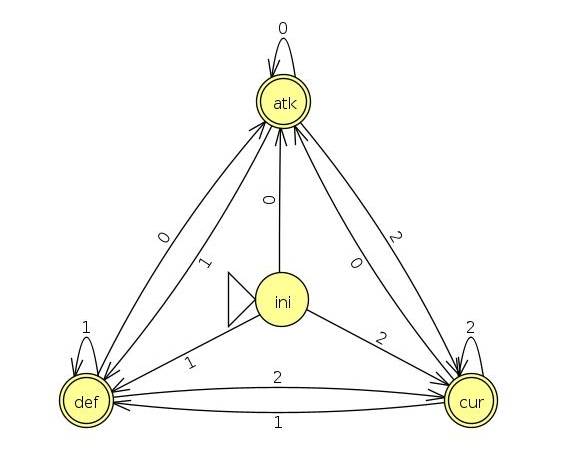
\includegraphics[width=0.50\linewidth]{combate.jpg}
\end{figure}

Essa máquina funciona de forma que, a partir de qualquer estado, uma entrada X só possa levar a um mesmo estado. Dessa forma, há um laço entre o estado e a entrada, sendo possível nomear um estado de acordo com a transição que leva até ele.
\newpage
\subsection{Automato de pilha}
\paragraph{}A Clase AutomatoDePilha abstrai um Automato de Pilha(AP), utilizando um vetor de caracteres para representar a pilha, e os métodos internos da pilha. Na inicialização do AP são passados os estados e transições, e utiliza o método interno "\_parse\_estados".
O método passa pelos estados e transições lidos do arquivo de entrada e retornado pelo método de leitura do AP.  Utilizando outras duas classes "Estado" e "Transicao",  para auxílio da verificação de qual transição pode ser realizada de acordo com a entrada e o caractere no topo da pilha.
\begin{minted}[breaklines]{python}
def _parse_estados(self, estados, transicoes):
    # Cria os estados e suas transicoes
    _estados = []
    saidas = [Saida.DEFESA,  Saida.CURA, Saida.ATAQUE]
    for estado in estados:
        transicoes_dict = []
        for transicao in transicoes:
            if estado.strip() == transicao[0].strip():
                _transicao = Transicao(
                    transicao[1][0], transicao[1][1], transicao[1][2], transicao[1][3])
                transicoes_dict.append(_transicao)

        _estado = Estado(estado, transicoes_dict, Saida.VAZIO if estado == self._nome_estado_inicial else saidas[int(transicao[1][0])])
        _estados.append(_estado)
    return _estados
\end{minted}
\subsubsection{O automato utilizado no combate:}
\textbf{O Automato de Pilha Utilizado no combate:}
\begin{figure}[!h]
  \centering
  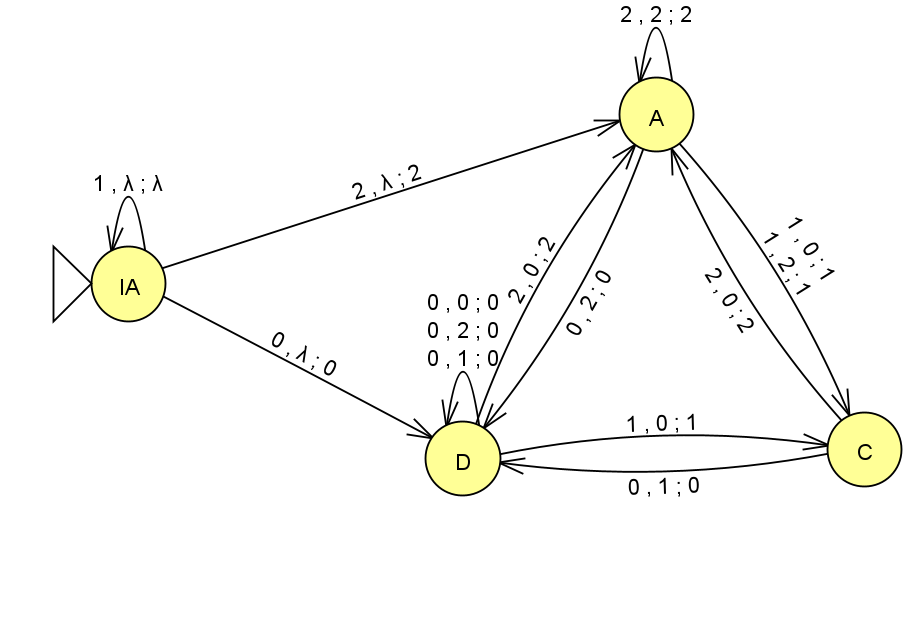
\includegraphics[width=0.5\linewidth]{Ap1.png}
\end{figure}
\newpage
\subsubsection{Realizando a transição no Automato de Pilha}
\paragraph{} Para realizar a transição existem dois cenários, com a pilha vazia e com a pilha cheia, ele verifica transição saindo do estado atual, e verifica qual a primeira que satisfaz o critério do símbolo a ser lido e do símbolo no topo da pilha, caso os dois requisitos sejam satisfeitos o novo estado atual passa a ser o estado de destino daquele estado, e retorna a saída do novo estado.

\begin{minted}[breaklines]{python}
def faz_transicao(self, entrada):
    # Realiza transicao da maquina
    estado = self._find_estado_atual()
    for transicao in estado.transicoes:
        if not self.pilha_vazia():
            if transicao.simbolo_a_ser_lido == entrada and transicao.simbolo_a_desempilhar == self._pilha[-1]:
                self._nome_estado_atual = transicao.estado_destino
                self._estado_atual = self._find_estado_atual()
                des = self.desempilha()
                if transicao.simbolo_a_empilhar != '*':
                    self.empilha(transicao.simbolo_a_empilhar)
                return self.get_saida_atual()
        else:
            if transicao.simbolo_a_ser_lido == entrada and transicao.simbolo_a_desempilhar == '*':
                self._nome_estado_atual = transicao.estado_destino
                self._estado_atual = self._find_estado_atual()
                if transicao.simbolo_a_empilhar != '*':
                    self.empilha(transicao.simbolo_a_empilhar)
                return self.get_saida_atual()
\end{minted}

\vspace{}
\paragraph{}Ao finalizar a transição, o simbolo de empilhamento está na última posição do vetor, o novo estado está na variável "\_estado\_atual" e a saída definida no estado é retornada para o combate. As próximas transições realizadas levarão em consideração as transições contidas no estado em questão.


\newpage

\subsection{Combate}
\paragraph{}A classe "Combate" representa um combate entre dois jogadores. O método "executa" inicia o combate, alternando os turnos entre os jogadores. Durante cada turno, os jogadores realizam ações com base nas transições das máquinas de estado. As ações incluem atacar e curar, dependendo das saídas das máquinas de estado. O combate continua até que um jogador tenha sua vida reduzida a zero, momento em que o vencedor é declarado com base na vida restante.

\begin{minted}[breaklines]{python}
class Combate:
    def __init__(self, player1, player2):
        self.player1 = player1
        self.player2 = player2
        self.turno = 0

    def executa(self):
        clear()

        # escolhe quem tem prioridade aleatoriamente
        player1 = random.choice([self.player1, self.player2])
        player2 = self.player1 if player1 == self.player2 else self.player2
\end{minted}

\section{Utilização}
Devido a não utilização de bibliotecas externas, não é necessária a instalação de nenhum dependência. A execução do código se dá pelo comando "python3 main.py". Ao executá-lo, um menu é apresentado com as opções de batalha.

\end{document}
